\begin{chapter}{Applications and Numerical Experiments}
\label{ch:numericalexperiments}
In the first part of the chapter we apply the algorithms to a variety of problems in image processing, computer vision, medical imaging and related fields.
The second part will be a comparison of the performance of the two implemented minimizer and close with with an numerical experiment investigating the 
dependence of the solution on the changes in the original picture. This is a first step in extending the IRLS algorithm towards recursive splitting into subdomain.\\

As briefly mentioned in the previous section, the test platform is a linux machine with two hyperthreaded 2.8GHz cores Intel i5-2520 (thus a total of four hardware threads)
with AVX vector extensions and 8 GB RAM. 


\section{Image denoising} % (fold)
\label{sec:image denoising}
The very basic application of the algorithm is of course denoising of common 2D grayscale or color pictures.
For grayscale pictures the TV minimization is performed over the Euclidian manifold $M=\mathbb{R}$, while for color
picture, as already explained in the introduction, we have either $M=\mathbb{R}^3$ for the linear-vectorial model or
$M=S^2\times\mathbb{R}$ for the non-linear chromaticity-brightness model.

\subsection{Grayscale} % (fold)
\label{sub:Grayscale}
% subsection Grayscale (end)

\FloatBarrier
\subsection{Color} % (fold)
\label{sub:Color}
In this example we perform the TV minimization of color images using the two different color models. In Figure \ref{fig:application_color1}
the among the image processing community well-known \emph{Lena} picture, which is rather small in size. Minimization in
the linear-vectorial color model using 5 IRLS iterations with one Newton step per reweighting is completed within $XXX$ seconds.\\

% subsection Color (end)
\begin{figure}[h!]
    \centering
    \subfloat[][Original]{
	\label{fig:application_color1_orig}
	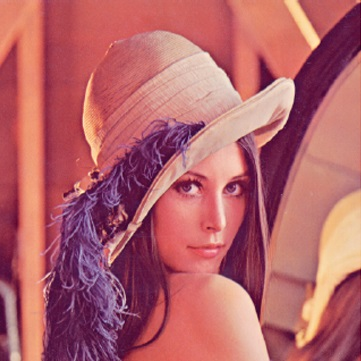
\includegraphics[width=0.325\linewidth]{./figures/experiments/Lena.jpg}
    }
    \subfloat[][Noisy]{
	\label{fig:application_color1_noise}
	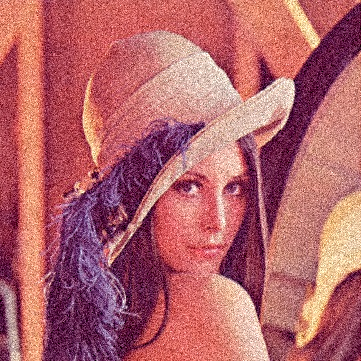
\includegraphics[width=0.325\linewidth]{./figures/experiments/Lena_noise.jpg}
    }
    \subfloat[][Denoised]{
	\label{fig:application_color1_denoised}
	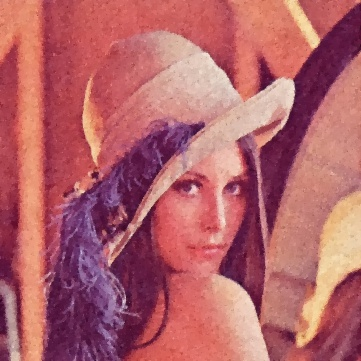
\includegraphics[width=0.325\linewidth]{./figures/experiments/denoised_Lena_noise.jpg}
    }\\
    \caption[Color image "Lena" linear vectorial denoising]{Denoising of a color images using the linear vectorial color model which corresponds to the manifold $\mathbb{R}^3$
	\subref{fig:application_color1_orig} Original image "Lena.jpg", $361\times 361$ px, 8 bit color depth
	\subref{fig:application_color1_noise} Componentwise gaussian noise $\mu=0$, $\sigma=?$ added
	\subref{fig:application_color1_denoised} Denoised, IRLS with $\lambda=?$, $5$ IRLS steps, $1$ newton steps per IRLS step
	\label{fig:application_color1}
    }
\end{figure}

Next, using the same model and parameters we denoise a different image with a size already in the megapixel range. The needed
time, however, is with $XXX$ seconds quite high. The result can be seen in Figure \ref{fig:application_color2}.\\

\begin{figure}[h!]
    \centering
    \subfloat[][Original]{
	\label{fig:application_color2_orig}
	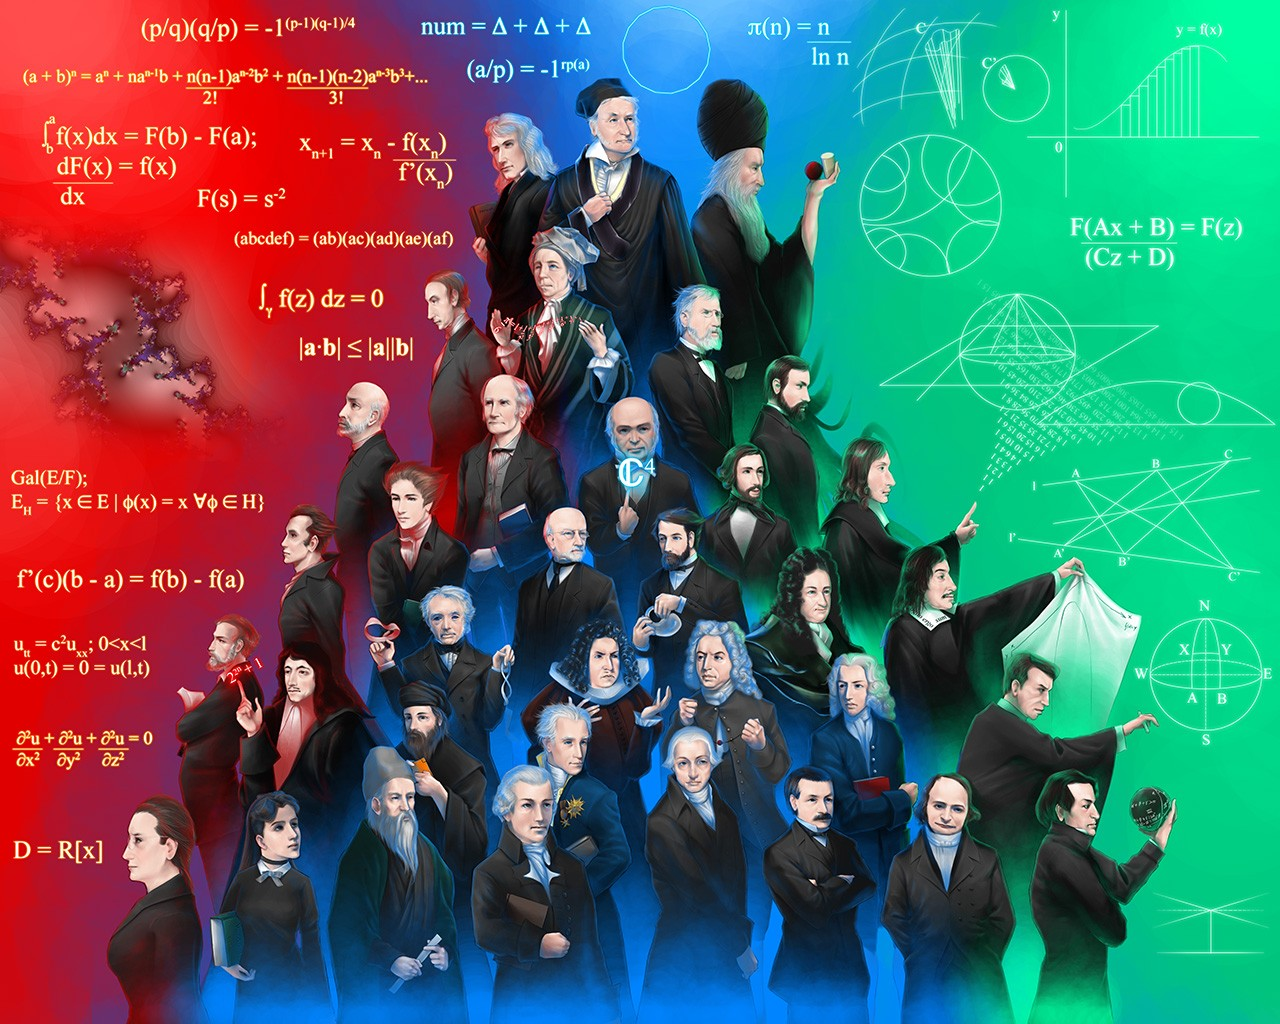
\includegraphics[width=0.325\linewidth]{./figures/experiments/mathematicians.jpg}
    }
    \subfloat[][Noisy]{
	\label{fig:application_color2_noise}
	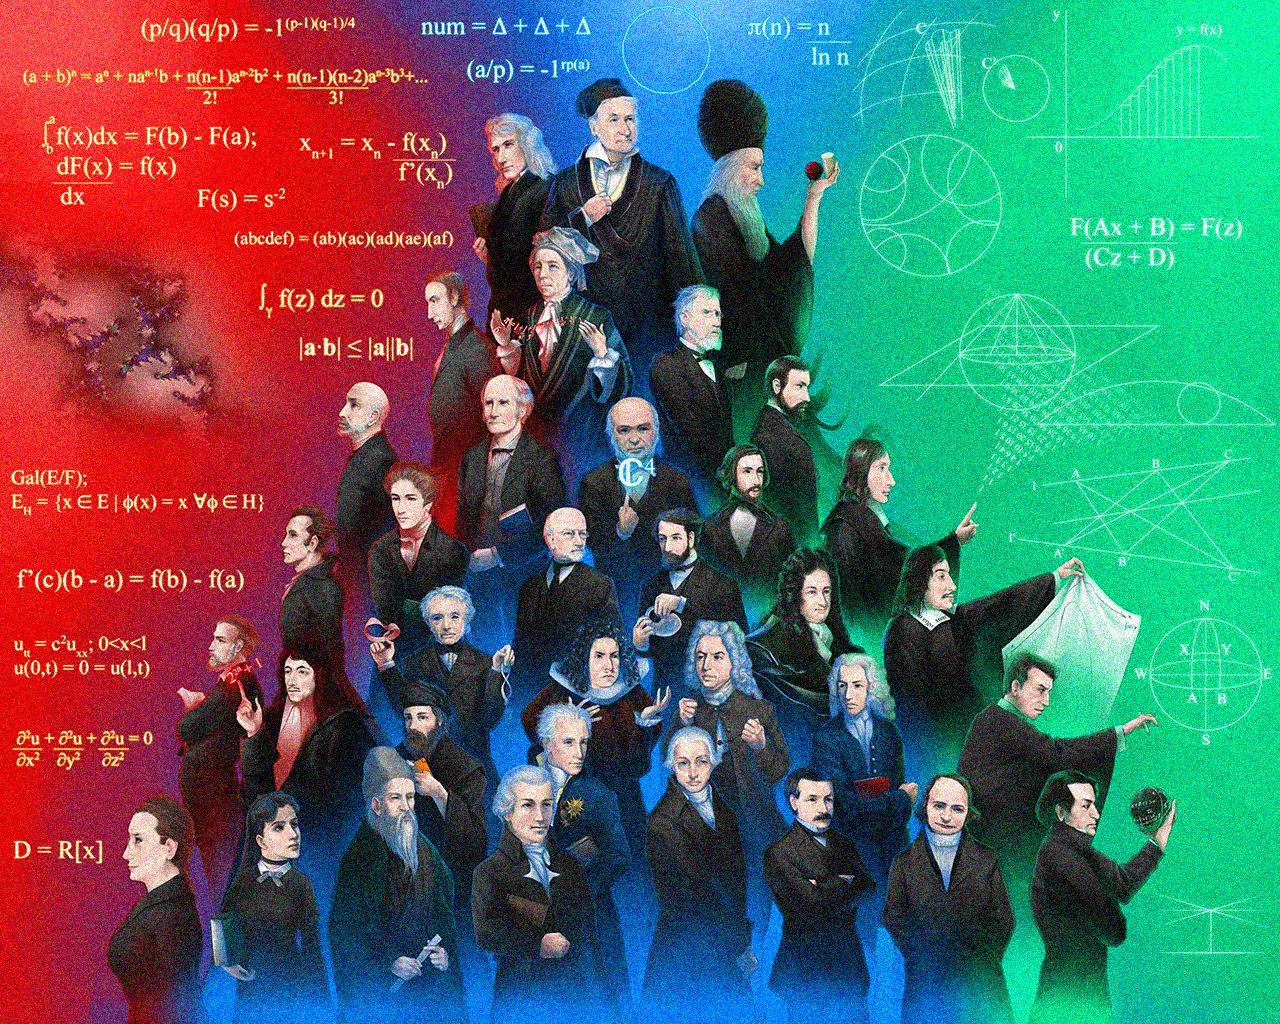
\includegraphics[width=0.325\linewidth]{./figures/experiments/noisy_mathematicians.jpg}
    }
    \subfloat[][Denoised]{
	\label{fig:application_color2_denoised}
	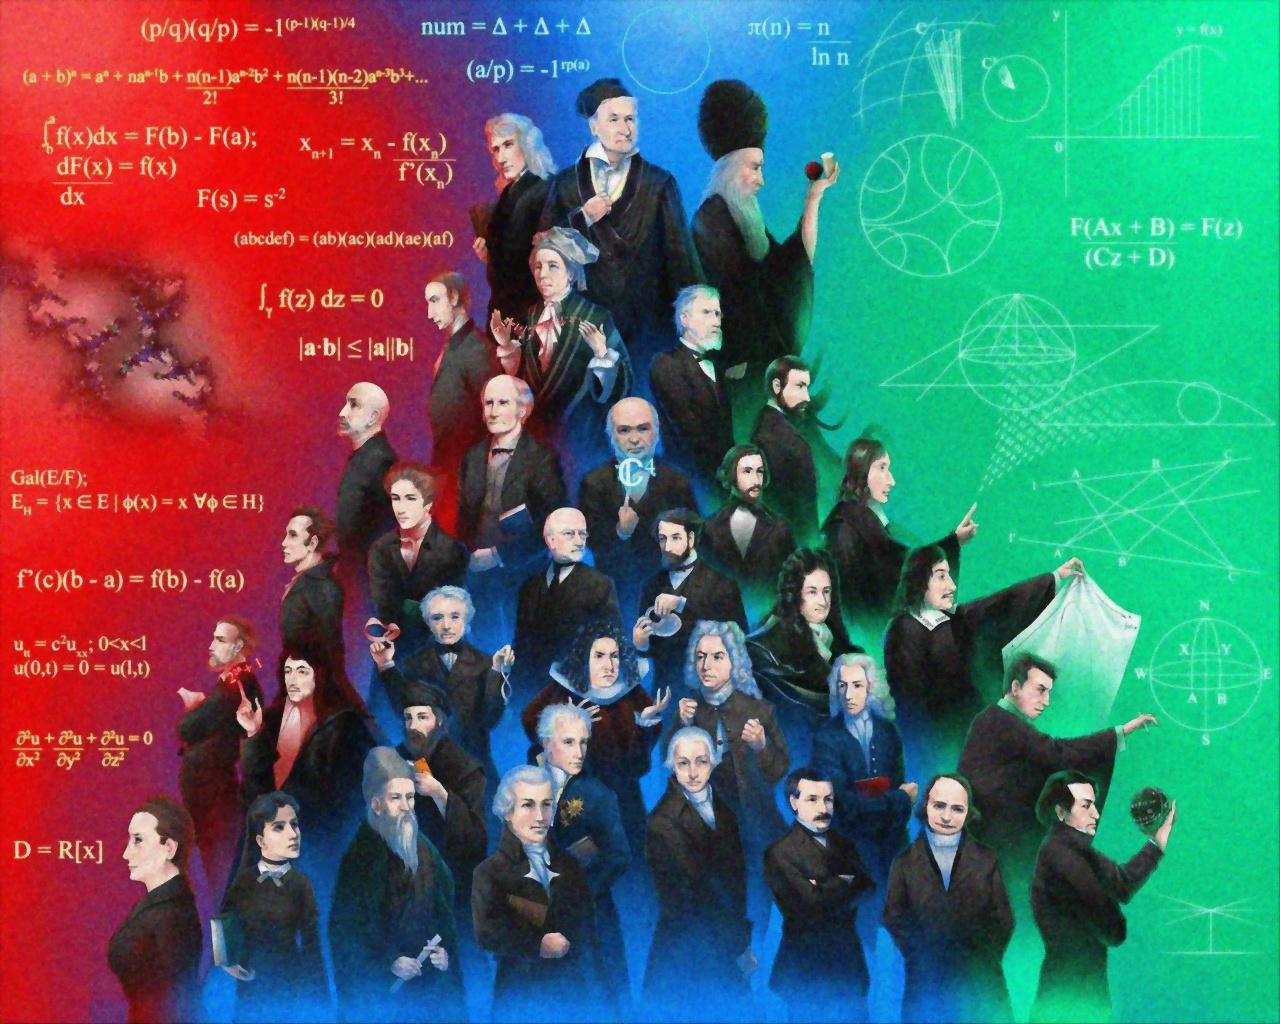
\includegraphics[width=0.325\linewidth]{./figures/experiments/denoised_noisy_mathematicians.jpg}
    }\\
    \caption[Large image "mathematicians" linear-vectorial denoising]{Denoising of a color images using the linear vectorial color model which corresponds to the manifold $\mathbb{R}^3$
	\subref{fig:application_color2_orig} Original image "mathematicians.jpg", $1280\times 1024$ px, 8 bit color depth
	\subref{fig:application_color2_noise} Componentwise gaussian noise $\mu=0$, $\sigma=?$ added
	\subref{fig:application_color2_denoised} Denoised, IRLS with $\lambda=?$, $?$ IRLS steps, $?$ newton steps per IRLS step
	\label{fig:application_color2}
    }
\end{figure}

Finally, in Figure \ref{fig:application_color3} we denoise a third picture using the chromaticity-brightness model. Here minimization over the product manifold
$S^2\times \mathbb{R}$ is performed by denoising the chromaticity($S^2$) and the brightness($\mathbb{R}$) separately, which has the added advantage of more 
fine-grained control over the process because two $\lambda$ parameters can be chosen separately for each part, too.


\FloatBarrier
\subsection{Inpainting} % (fold)
We consider a damaged picture were a considerable part of the picture has been overpainted with blue color. In the first step we detect the damaged region which in this
case is done via a simple color selector (e.g. all pixels with a blue value larger than 0.95). In principle many other selection methods known from common raster graphic editors
could be implemented here as well. \\
Next, the a first guess is calculated using scattered linear interpolation and lastly the TV minimization itself is performed. The process is summarized in Figure 
\ref{fig:application_colorinpaint1}.

\label{sub:Inpainting}
\begin{figure}[h!]
    \centering
    \subfloat[][Original]{
	\label{fig:application_colorinpaint1_orig}
	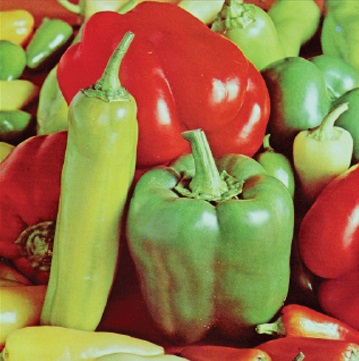
\includegraphics[width=0.25\linewidth]{./figures/experiments/Pepper.jpg}
    }
    \subfloat[][Damaged]{
	\label{fig:application_colorinpaint1_dam}
	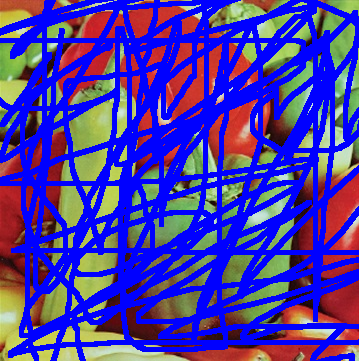
\includegraphics[width=0.25\linewidth]{./figures/experiments/Pepper_dam.png}
    }
    \subfloat[][First guess]{
	\label{fig:application_colorinpaint1_guess}
	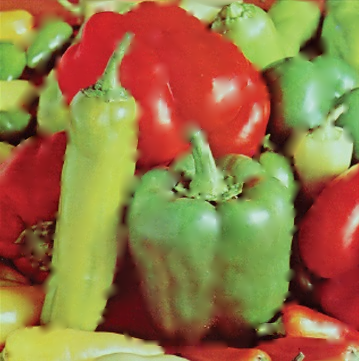
\includegraphics[width=0.25\linewidth]{./figures/experiments/firstguess_Pepper_dam.png}
    }
    \subfloat[][Restored]{
	\label{fig:application_colorinpaint1_restored}
	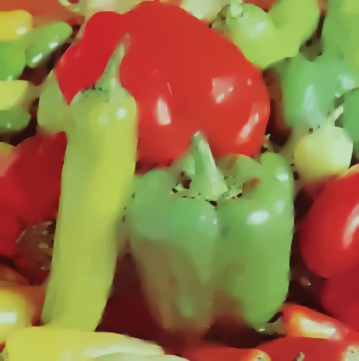
\includegraphics[width=0.25\linewidth]{./figures/experiments/denoised_Pepper_dam.png}
    }\\
    \caption[Denoising linear vectorial]{Denoising of a color images using the linear vectorial color model which corresponds to the manifold $\mathbb{R}^3$
	\subref{fig:application_colorinpaint1_orig} Original image "Pepper.png", $359\times 361$ px, 8 bit color depth
	\subref{fig:application_colorinpaint1_dam} Damaged by overpainting with blue color
	\subref{fig:application_colorinpaint1_guess} First guess via componentwise scattered interpolation
	\subref{fig:application_colorinpaint1_restored} Restored, IRLS with $\lambda=?$, $?$ IRLS steps, $?$ newton steps per IRLS step
	\label{fig:application_colorinpaint1}
    }
\end{figure}

% subsection Inpainting (end)


\FloatBarrier
\subsection{Recolorization} % (fold)
Colarization, also known is color inpainting, because it is basically just a special of inpainting is performed in the next example.
Here the picture is not necessarily noisy but we assume only the brightness of each pixel is known, while the chromaticity is known only for a low ratio $r=0.01$ of all pixels.
Note that this splitting implies that inpainting and TV minimization takes place only $S^2$.\\

As in the previous example, we first have to detect all damaged, i.e. non-colored, pixels to inpaint. Again we use scattered interpolation to obtain the first guess which is depcited
in Figure \ref{fig:application_colorinpaint1} \subref{fig:application_colorinpaint1_guess}. One can observe that the color runs over the edges of leafes. To avoid this we need to
detect the edges in the brightness part using the Canny edge detector \cite{Canny}, for example, and set the edge weights for the chromaticity part accordingly. As a result, we indeed
obtain sharp and clear edges in the final result \ref{fig:application_colorinpaint1} \subref{fig:application_colorinpaint1_restored}.

\label{sub:Recolorization}
\begin{figure}[h!]
    \centering
    \subfloat[][Original]{
	\label{fig:application_colorization1_orig}
	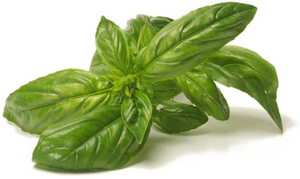
\includegraphics[width=0.25\linewidth]{./figures/experiments/Basil.jpg}
    }
    \subfloat[][Colors removed]{
	\label{fig:application_colorization1_colorless}
	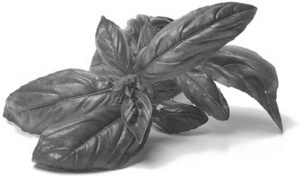
\includegraphics[width=0.25\linewidth]{./figures/experiments/colorless_Basil.jpg}
    }
    \subfloat[][First guess]{
	\label{fig:application_colorization1_guess}
	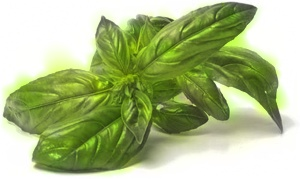
\includegraphics[width=0.25\linewidth]{./figures/experiments/recolored_fg_Basil.jpg}
    }
    \subfloat[][Recolored]{
	\label{fig:application_colorization1_restored}
	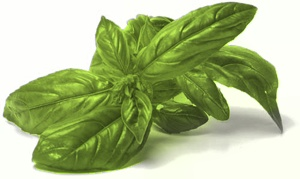
\includegraphics[width=0.25\linewidth]{./figures/experiments/recolored_Basil.jpg}
    }\\
    \caption[Recolorization]{Recolorization using color inpainting in the Chromaticity-Brightness color model, corresponding to $S^2\times\mathbb{R}$
	\subref{fig:application_colorization1_orig} Original image "Basil.jpg", $300\times 179$ px, 8 bit color depth
	\subref{fig:application_colorization1_colorless} Image with a ratio of approximately $0.01$ remaining colored pixels
	\subref{fig:application_colorization1_guess} First guess via componentwise scattered interpolation
	\subref{fig:application_colorization1_restored} Recolored, IRLS with $\lambda=?$, $?$ IRLS steps, $?$ newton steps per IRLS step
	\label{fig:application_colorization1}
    }
\end{figure}
% subsection Recolorization (end)

\FloatBarrier
\subsection{Volume images} % (fold)
\label{sub:Volume images}
We conclude the picture section with an example of a 3D volume image as they might occur in medical imaging from magnetic resonance imaging (MRI) or
computed tomography. In this demonstration, however, we chose the example of the so-called \emph{Boston teapot}, taken a volume image library \cite{volumeLib}
and added componentwise gaussian noise. The image represents only intensity values, hence minimization is performed over $\mathbb{R}$. The result are shown
in Figure \ref{fig:application_volume1_orig}.\\

For this picture we used the proximal point algorithm, because the memory and computational requirements of the IRLS for a picture of this size are very high:
In section \label{sub:NewtonequationfortheTVfunctional} it was shown that the dimension of the sparse linear system is $\operatorname{dim}(M)XYZ$ which
in this case amounts to $1.1\times 10^{7}$, which is the length of the gradient while the Hessian will contain $7.7\times 10^{7}$ non-zero-entries.
The solution of a sparse linear system of that size is computationally very demanding while in comparison the geodesic averaging and karcher mean calculations
simplify to mostly vectorized addition and subtraction operations on a simple manifold like $\mathbb{R}$.

\begin{figure}[h!]
    \centering
    \subfloat[][Original]{
	\label{fig:application_volume1_orig}
	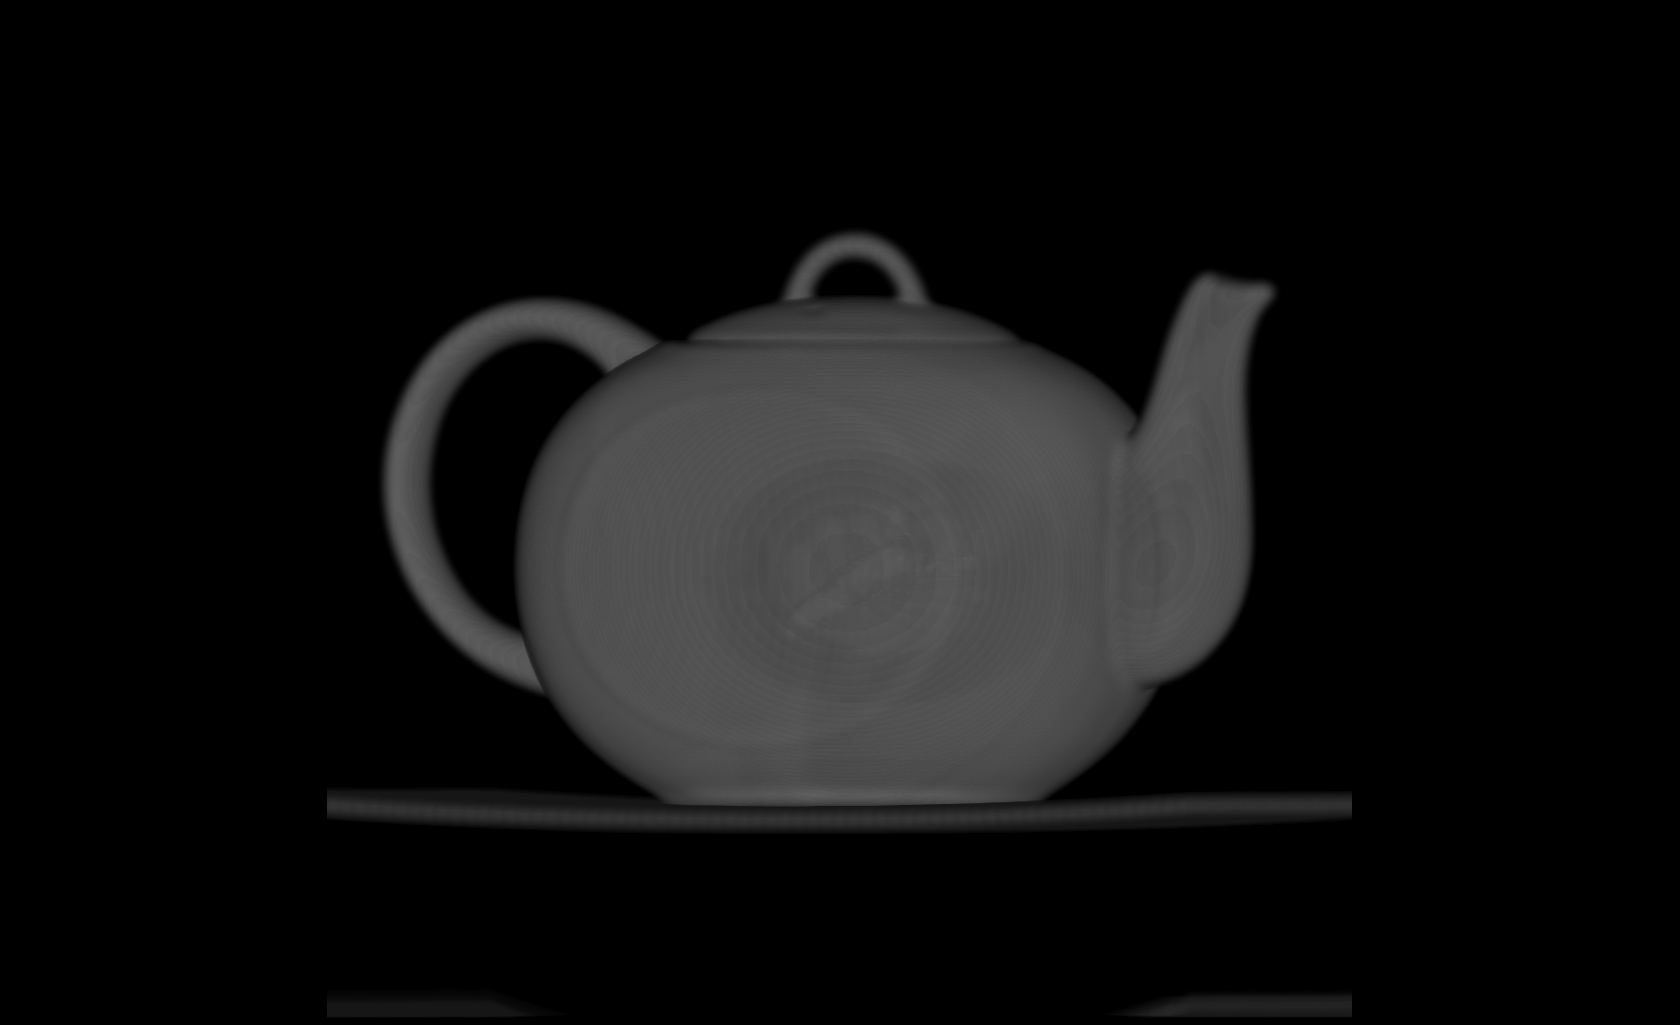
\includegraphics[width=0.325\linewidth]{./figures/experiments/VolumeImg.png}
    }
    \subfloat[][Noisy]{
	\label{fig:application_volume1_noise}
	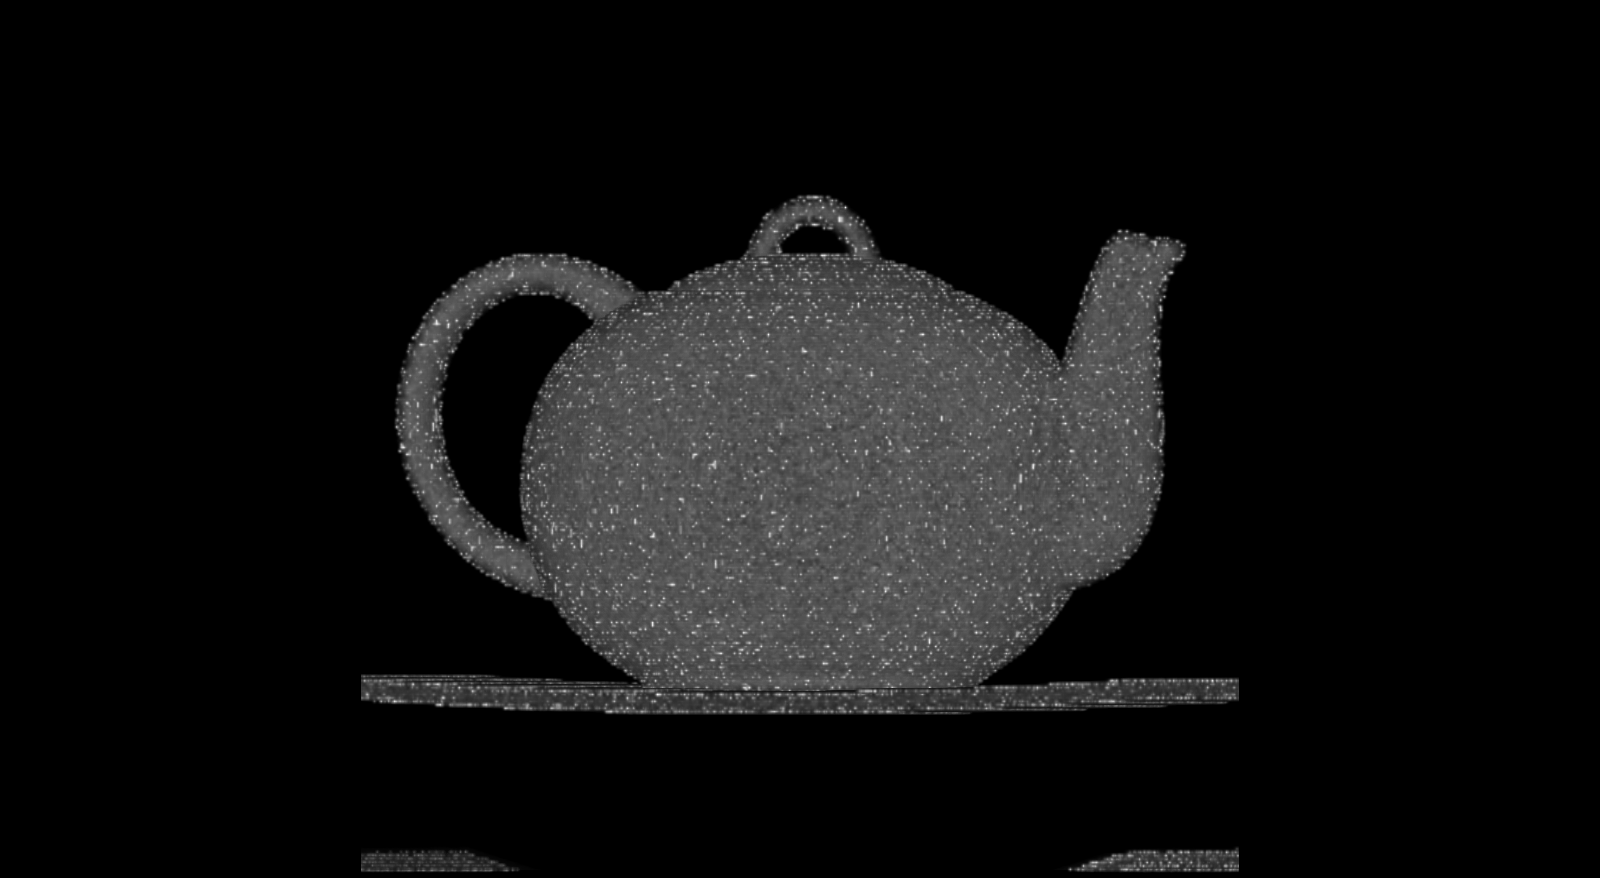
\includegraphics[width=0.325\linewidth]{./figures/experiments/noisyVolumeImg.png}
    }
    \subfloat[][Denoised]{
	\label{fig:application_volume1_denoised}
	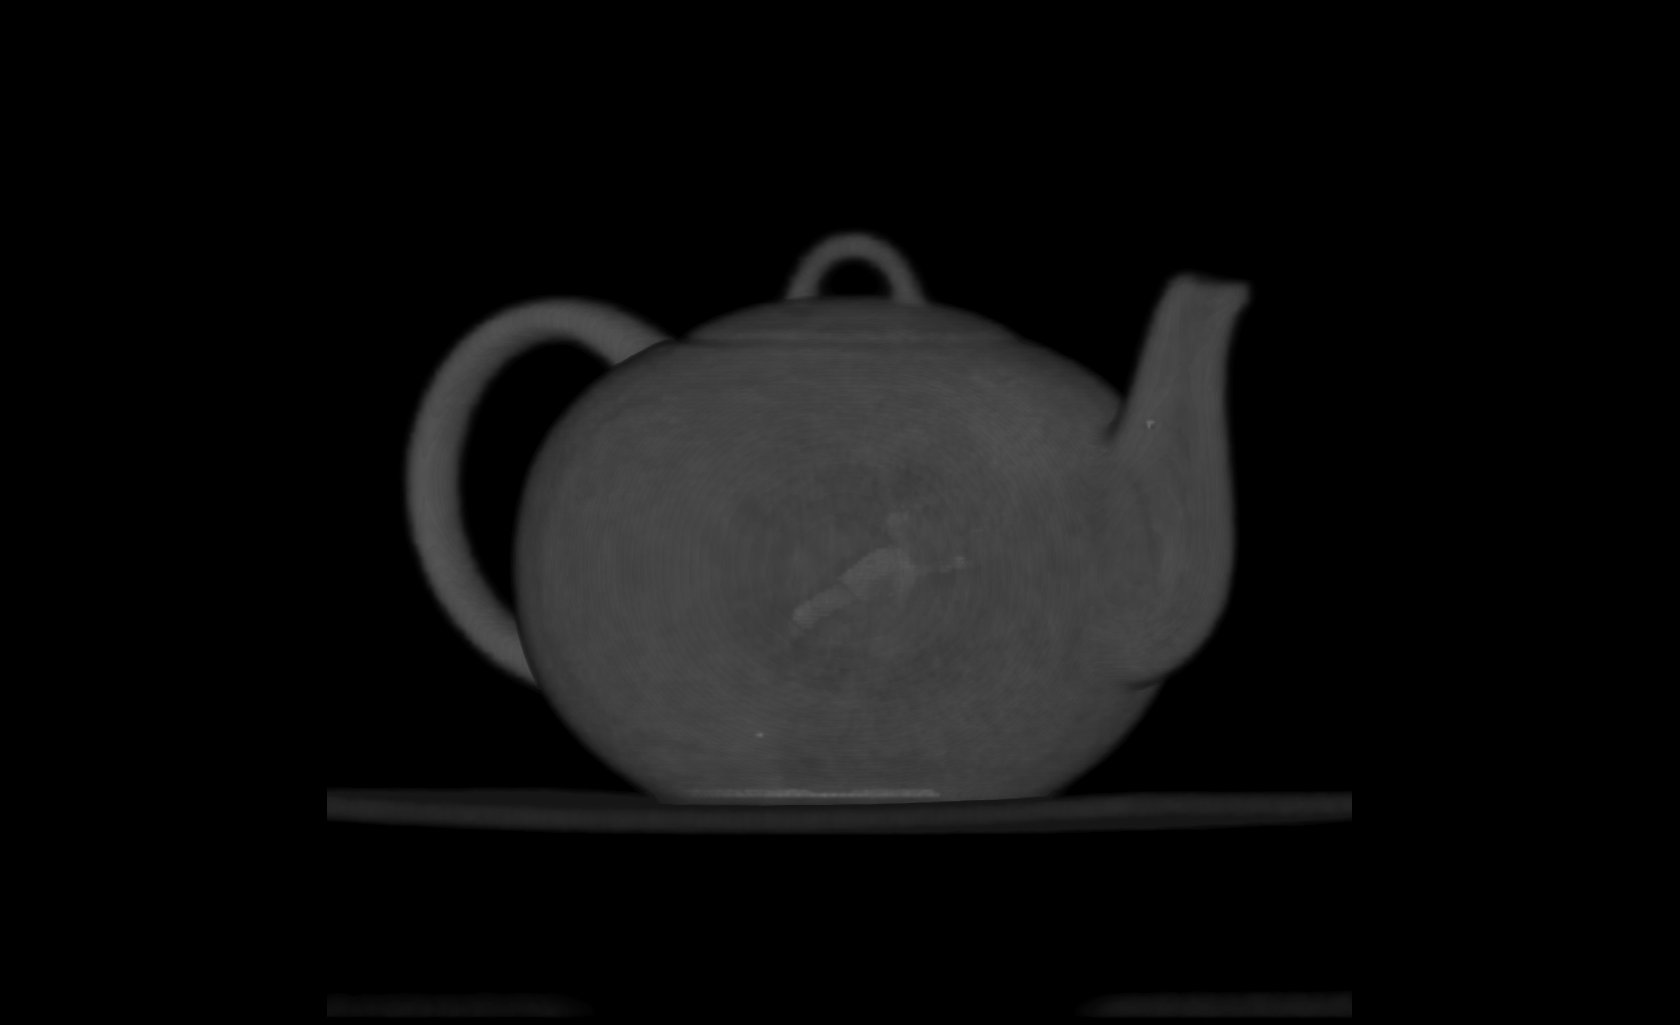
\includegraphics[width=0.325\linewidth]{./figures/experiments/denoisedVolumeImg.png}
    }\\
    \caption[Denoising 3D Grayscale Volume Data]{Denoising a 3D graysclae volume image
	\subref{fig:application_volume1_orig} Original image "BostonTeapot.raw", $256\times 256 \times 178$ px, 8 bit color depth
	\subref{fig:application_volume1_noise} Componentwise gaussian noise $\mu=0$, $\sigma=?$ added
	\subref{fig:application_volume1_denoised} Denoised, Proximal point with $\lambda=?$, $50$ PRPT steps
	\label{fig:application_volume1}
    }
\end{figure}
% subsection Volume images (end)

% section Color image denoising (end)

\FloatBarrier
\section{SO(2) and SO(3) images data} % (fold)
\label{sec:SO images data}

\subsection{Synthetic data} % (fold)
\label{sub:Synthetic data}
The following synthetic $SO(3)$ image is constructed in the following way. Let $\Omega=\lbrace 1,\ldots,30 \rbrace^2$ and define for every $(i,j)\in\Omega$
a rotation axis
\begin{equation}
	v = \begin{cases}
	    (2x,y,0)^{T}, & x>0.5\\
	    (0,2x,0.5)^{T}, & \text{ else}
	\end{cases},
\end{equation}
where $x=\frac{j}{30}, y=\frac{i}{30}$ and a rotation angle
\begin{equation}
    \alpha = \begin{cases}
	   x + y, & x > y\\
	   \frac{\pi}{2} + x - y, \text{ else}
    \end{cases}.
\end{equation}
Then assign the corresponding $SO(3)$ element representing a rotation by $\alpha$ and about $v$. Noise is added componentwise and the noisy matrix is
then projected back to $SO(3)$ using a the projector $P_{SO(n)}(A)=UV^{T}$ where $A=U\Sigma V^T$ is the singular value decomposition of $A$.

\begin{figure}[h!]
    \centering
    \subfloat[][Original]{
	\label{fig:application_so1_orig}
	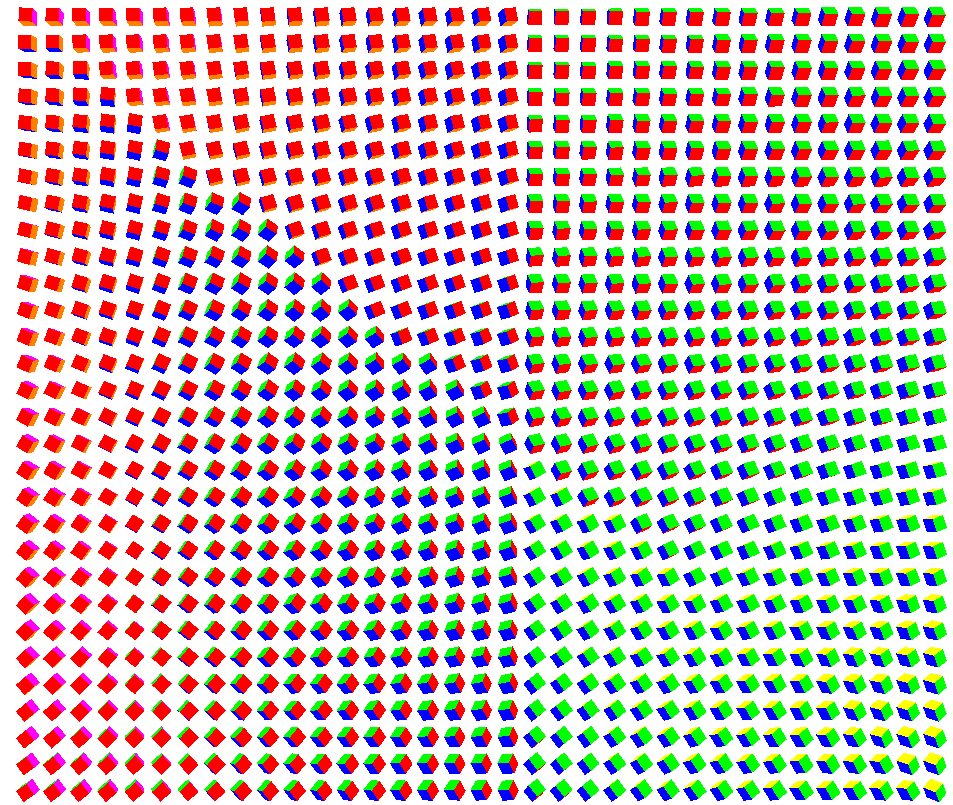
\includegraphics[width=0.325\linewidth]{./figures/experiments/son30x30original.png}
    }
    \subfloat[][Damaged]{
	\label{fig:application_so1_dam}
	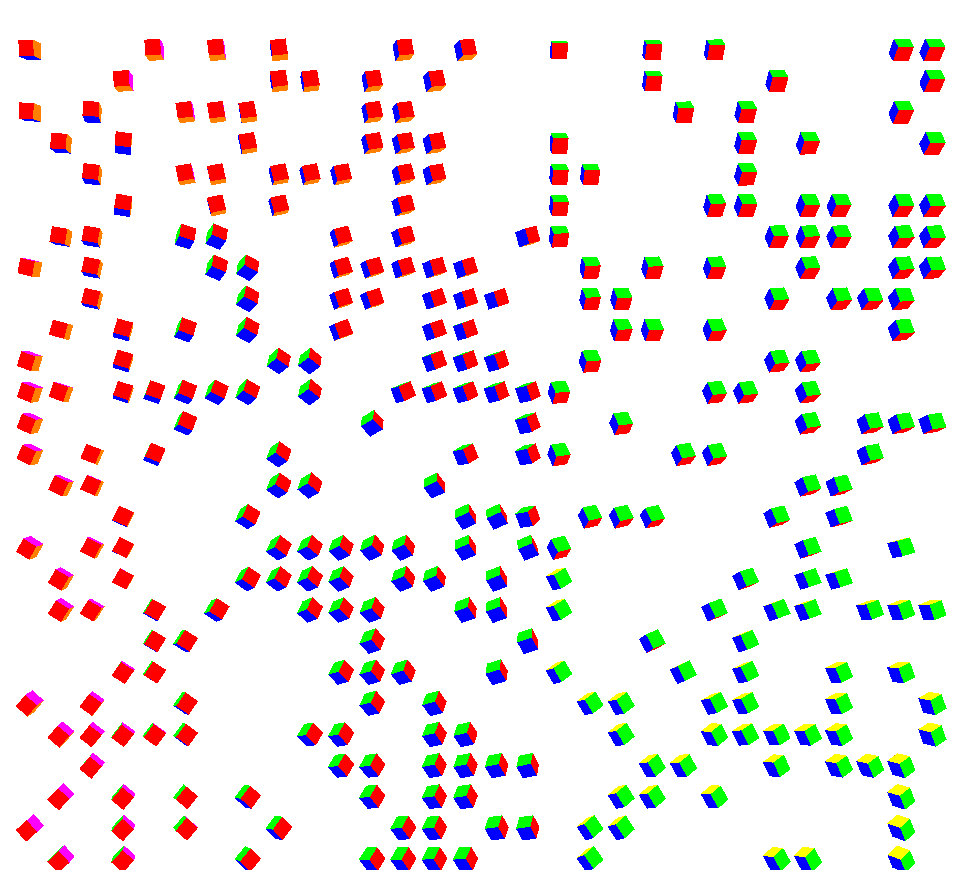
\includegraphics[width=0.325\linewidth]{./figures/experiments/son30x30damaged.png}
    }
    \subfloat[][Reconstructed]{
	\label{fig:application_so1_inp}
	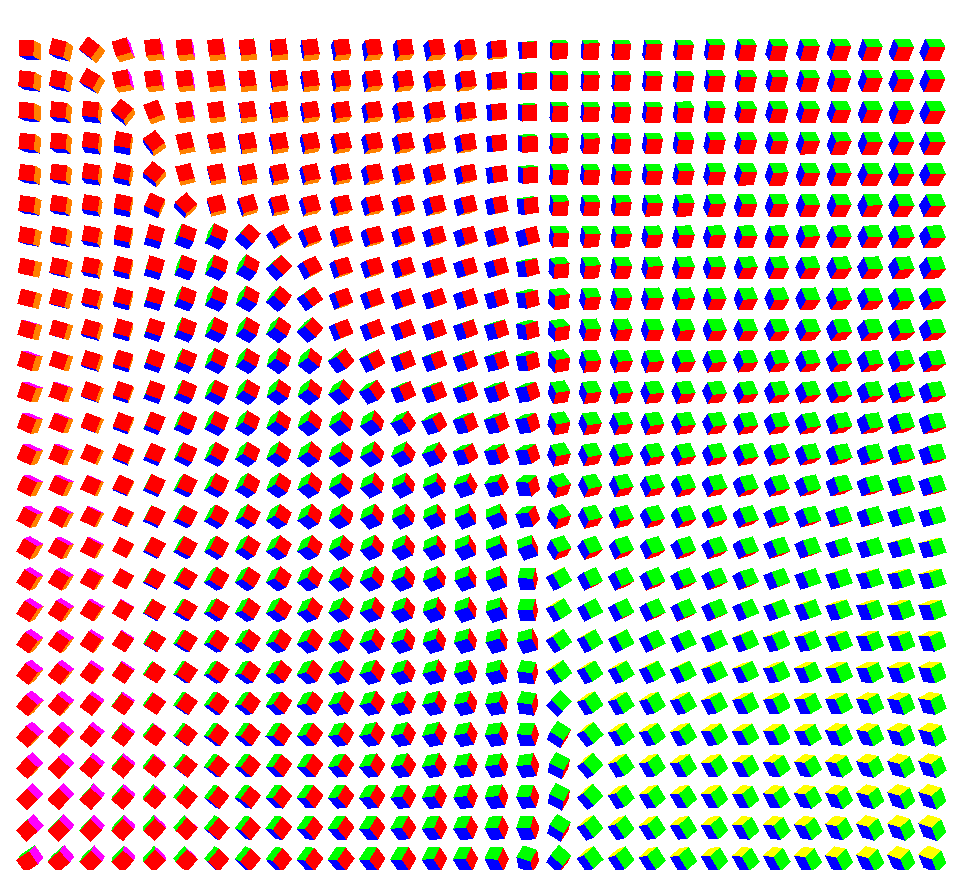
\includegraphics[width=0.325\linewidth]{./figures/experiments/son30x30inpainted.png}
    }\\
    \caption[Inpainting of synthetic SO(3) picture]{Inpainting of synthetic SO(3) picture
	\subref{fig:application_so1_orig} Original image: Synthetic, nonsmooth SO(3), $30\times 30$ px
	\subref{fig:application_so1_dam} Threshold $p=?$
	\subref{fig:application_so1_inp} Denoised, IRLS with $\lambda=?$, 5 IRLS steps, 1 Newton step per IRLS
	\label{fig:application_so1}
    }
\end{figure}

% subsection Synthetic data (end)

\FloatBarrier
\subsection{Fingerprint orientation data} % (fold)
\label{sub:Fingerprint orientation data}
Fingerprint matching is  based on extracting a set of particular features, called \emph{minutiae}, which uniquely define the fingerprint.
These features are usually ridge endpoint or ridge bifurkation points that are saved along with their position and orientation. This
means that prior to minutia detection and extraction the calculation of an orientation field is necessary.\\

For pictures of fingerprint this is just a special form of edge detection which can be done by calculating Sobel derivatives for every pixel.
Depending on the quality and noise level of the picture the computed orientation field can be very noisy itself which is another application
for our TV algorithms.\\

% subsection Fingerprint orientation data (end)
\begin{figure}[h!]
    \centering
    \subfloat[][Original]{
	\label{fig:application_fingerprint1_orig}
	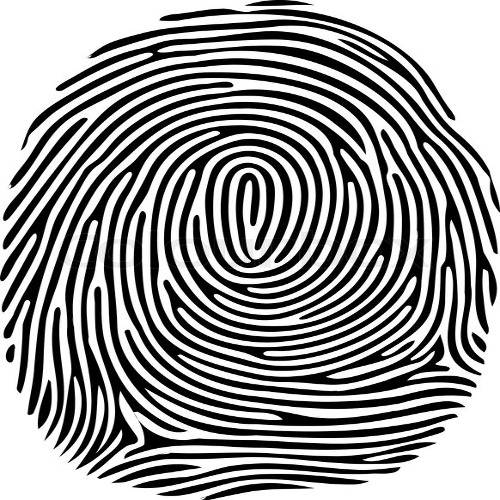
\includegraphics[width=0.325\linewidth]{./figures/experiments/fingerprint4.jpg}
    }
    \subfloat[][Computed Orientation field]{
	\label{fig:application_fingerprint1_noise}
	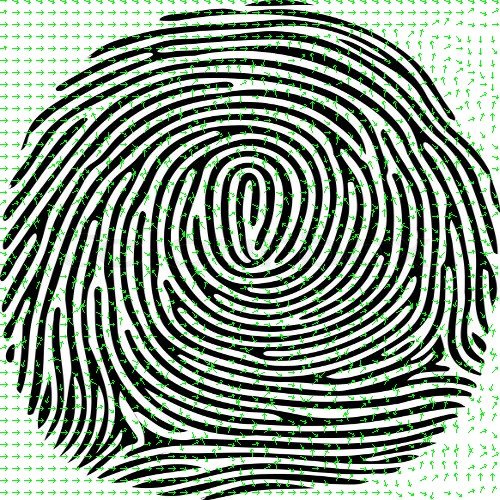
\includegraphics[width=0.325\linewidth]{./figures/experiments/input_fingerprint4.jpg}
    }
    \subfloat[][Denoised Orientation field]{
	\label{fig:application_fingerprint1_denoised}
	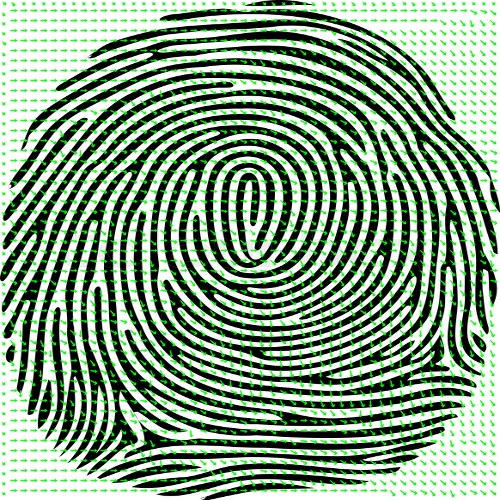
\includegraphics[width=0.325\linewidth]{./figures/experiments/denoised_fingerprint4.jpg}
    }\\
    \caption[Fingerprint orientation denoising]{Denoising a orientation field from a fingerprint, orientations represented by SO(2) elements
	\subref{fig:application_fingerprint1_orig} Original fingerprint 
	\subref{fig:application_fingerprint1_noise} Orientation field computed using Sobel derivatives PLACEHOLDER
	\subref{fig:application_fingerprint1_denoised} Denoised, IRLS with $\lambda=?$, $?$ IRLS steps, $?$ Newton steps per IRLS step PLACEHOLDER
	\label{fig:application_fingerprint1}
    }
\end{figure}

\FloatBarrier
\subsection{Reconstruction of a dense optical flow field} % (fold)
\label{sub:reconstructionDenseOpticalFlow}
An optical flow is the pattern of apparent motion between two consecutive frame of a video sequence. This may be the result of either an actual movement of the depicted object
or the result of a moving camera. Important applications are for example (anormal) motion detection, crowd behavior analysis, surveillance, video compression or image segmentation.\\
A \emph{dense} optical flow field can be interpreted as a vector field where each vector describes the displacement of a point between from one frame to the next. If
the set of points is retricted to only a few points of interest, a sparse feature set, we have \emph{sparse} optical flow.\\

In the following example, we only use a sparse feature set for tracking and flow computation in a short video sequence. The traffic scene was taken from a crowds/high density moving object data 
set provided by \cite{AliShah}. At first, we compute the sparse optical flow using the Lucas-Kanade algorithm \cite{LucasKanade} implemented in the OpenCV library. \\
For the set of tracked features 
$\mathcal{F}_1:=\lbrace{F^{(1)}_i\rbrace}_{i=1}^{400}\subset\Omega\subset\mathbb{R}^2$ in the first frame the algorithm tries to identify each feature in the second frame resulting in a set of
identified features $\mathcal{F}_2:=\lbrace{F^{(2)}_i\rbrace}_{i=1}^{N<400}\subset\Omega\subset\mathbb{R}^2$ and corresponding displacement vectors 
$\mathcal{V}_{12}:=\lbrace{V_i\,|\,V_i=F_i^{(2)}-F_i^{(1)}\rbrace}_{i=1}^{N}$.\\

We now assign to each pixel in our data an SO(2) element in the following way
\begin{align}
    \alpha_i &=\arctan\left(\frac{V^y_i}{V^x_i}\right) \\
    I(i,j) &= 
    \begin{cases}
    	\begin{pmatrix}
	    \cos\alpha_i    & -\sin\alpha_i\\
	    \sin\alpha_i    & \cos\alpha_i
	\end{pmatrix} & (i,j)\in \mathcal{F}_{2} \\
	0 & \text{ otherwise}
    \end{cases}
\end{align}

Since we want to reconstruct the dense flow, this is an inpainting problem and we have to perform scattered interpolation before running the algorithm. The result can be seen in 
Figure \ref{fig:application_flowfield1}.
\begin{figure}[h!]
    \centering
    \subfloat[][Original]{
	\label{fig:application_flowfield1_orig}
	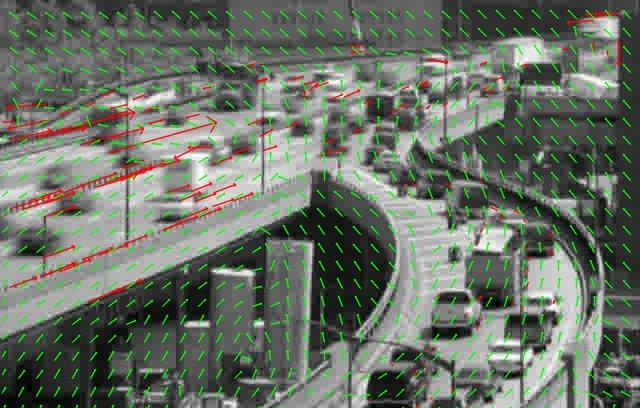
\includegraphics[width=0.325\linewidth]{./figures/experiments/reconstructed_optical_flow.jpg}
    }
    \subfloat[][Computed Sparse Flow field]{
	\label{fig:application_flowfield1_noise}
	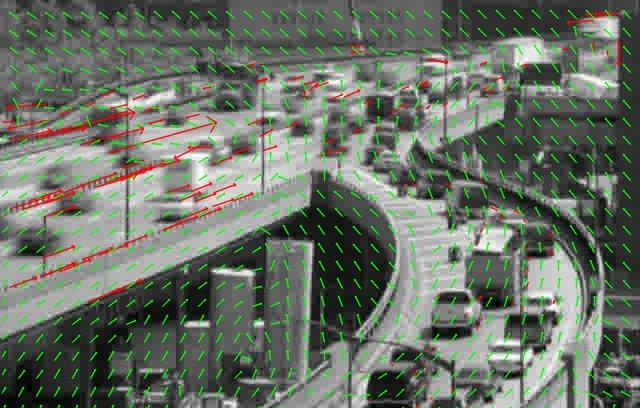
\includegraphics[width=0.325\linewidth]{./figures/experiments/reconstructed_optical_flow.jpg}
    }
    \subfloat[][Reconstructed orientation field]{
	\label{fig:application_flowfield1_denoised}
	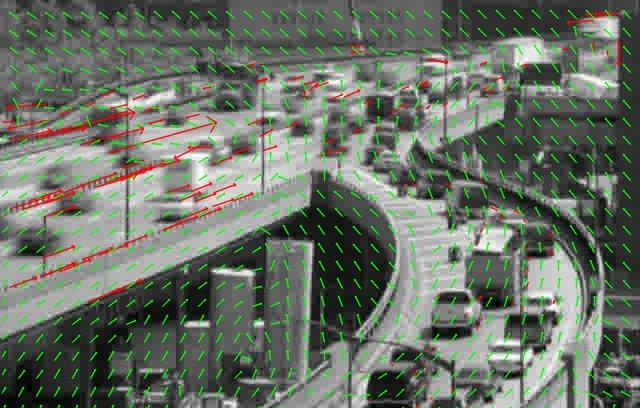
\includegraphics[width=0.325\linewidth]{./figures/experiments/reconstructed_optical_flow.jpg}
    }\\
    \caption[Dense optical flow reconstruction]{Reconstructing a dense flow from sparse feature tracking, orientations represented by SO(2) elements
	\subref{fig:application_flowfield1_orig} Frame of original video scene PLACEHOLDER
	\subref{fig:application_flowfield1_noise} Sparse features tracked using PLACEHOLDER
	\subref{fig:application_flowfield1_denoised} Reconstructed, IRLS with $\lambda=?$, $?$ IRLS steps, $?$ Newton steps per IRLS step
	\label{fig:application_flowfield1}
    }
\end{figure}

Of course the optimization could have also been performed on $S^1$. Furthermore, there is also a more direct, variational approach for the calculation of the flow field
which is also based on TV minimization but has a different fidelity term. This is one possibility for further extension of the library and is discussed in more detail in 
section \ref{sec:Extensions}

% subsection Calculation of a dense flow field (end)

% section SO(3) images data (end

\FloatBarrier
\section{SPD(3) image data} % (fold)
\label{sec:SPD(3) image data}

\subsection{Synthetic data} % (fold)
\label{sub:Synthetic data}
For the construction of the synthetic $SPD(3)$ image in Figure \ref{fig:application_spd1}, let $\Omega=\lbrace 1,\ldots,n \rbrace^2$ and define for every $(i,j)\in\Omega$
a rotation axis
\begin{equation}
	v = \begin{cases}
	    (x,y,2)^{T}, & x+y<1\\
	    (y,-x,1)^{T}, & \text{ else}
	\end{cases},
\end{equation}
where $x=\frac{j}{n}, y=\frac{i}{n}$ and a rotation angle
\begin{equation}
    \alpha = \begin{cases}
	   x+2y, & x+y<1\\
	   y+2x, \text{ else}
    \end{cases}.
\end{equation}
Let $R$ be the corresponding $SO(3)$ element representing a rotation by $\alpha$ and about $v$. Then define a diagonal matrix $D=\operatorname{diag}(x+0.2,y+0.2,0.5)$
and finally assign the matrix $A=R^{T}DR$ to the pixel.\\
Noise is then added by taking the matrix logarithm of every pixel, adding gaussian componentwise noise and apply the matrix exponential again.
\begin{figure}[h!]
    \centering
    \subfloat[][Original]{
	\label{fig:application_spd1_orig}
	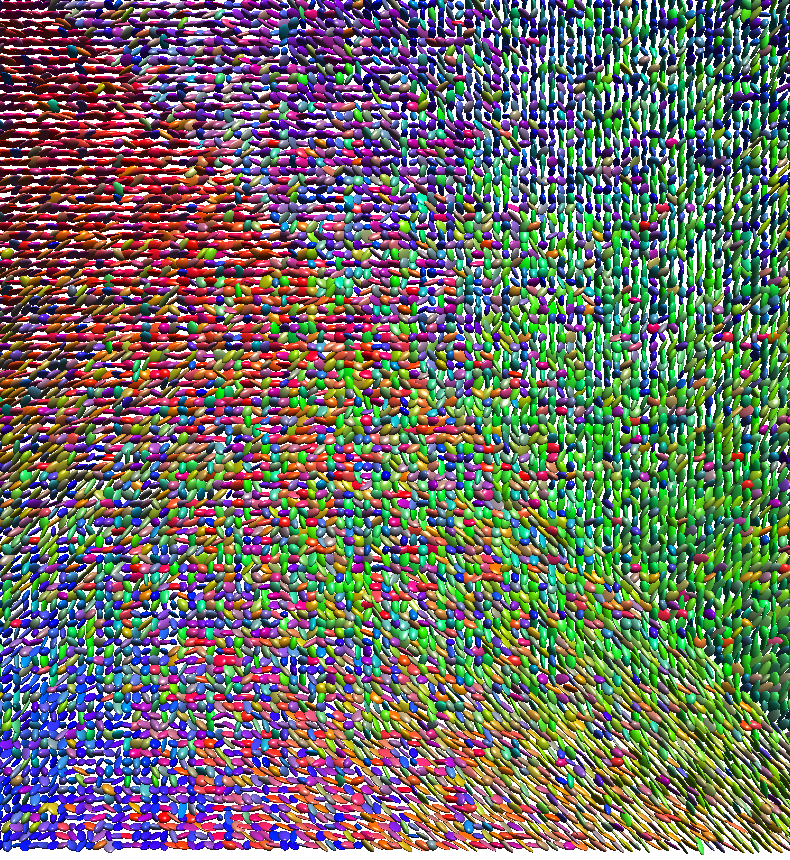
\includegraphics[width=0.325\linewidth]{./figures/experiments/noisy_spd100x100.png}
    }
    \subfloat[][Damaged]{
	\label{fig:application_spd1_noise}
	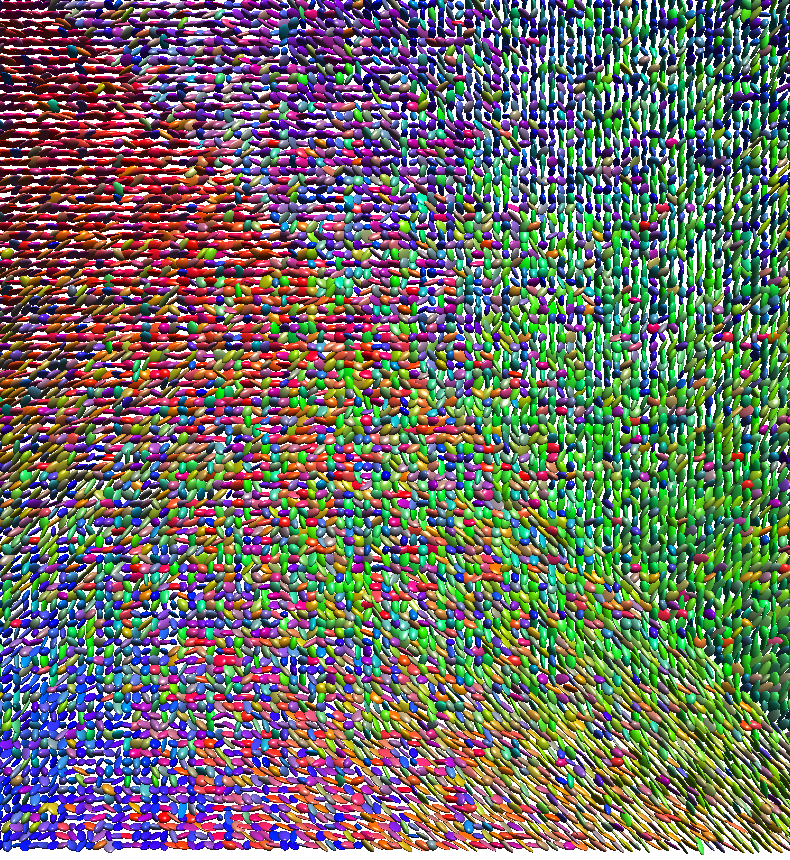
\includegraphics[width=0.325\linewidth]{./figures/experiments/noisy_spd100x100.png}
    }
    \subfloat[][Denoised]{
	\label{fig:application_spd1_denoised}
	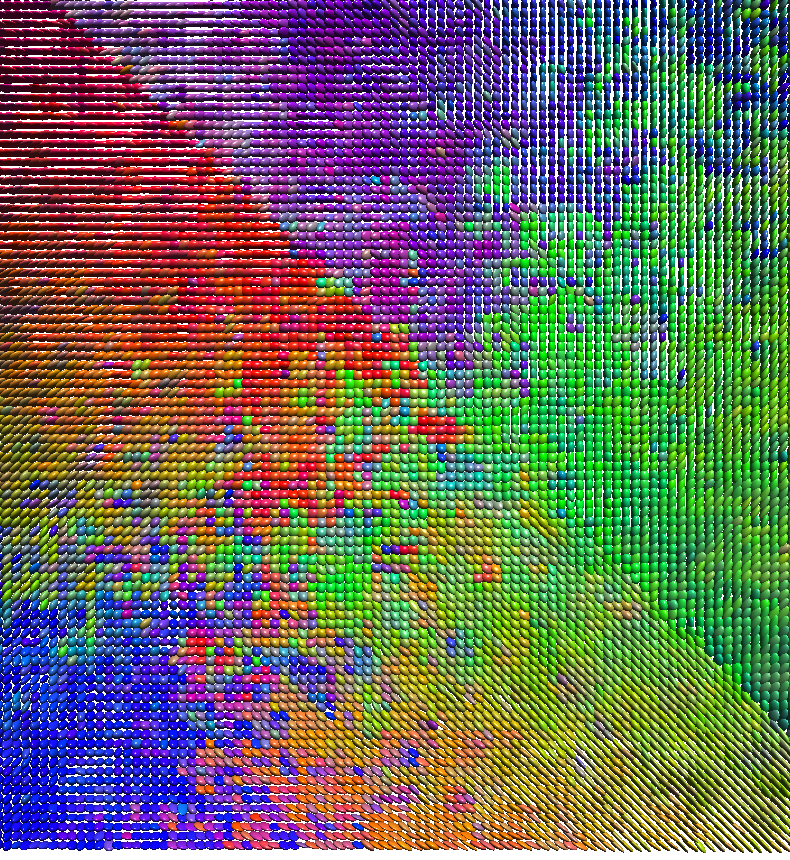
\includegraphics[width=0.325\linewidth]{./figures/experiments/denoised_spd100x100.png}
    }\\
    \caption[Denoising of synthetic SPD(3) picture]{Denoising of synthetic SPD(3) picture
	\subref{fig:application_spd1_orig} Original image: Synthetic, nonsmooth SPDO(3), $100\times 100$ px PLACEHOLDER
	\subref{fig:application_spd1_noise} Threshold $p=?$
	\subref{fig:application_spd1_denoised} Denoised, IRLS with $\lambda=?$, 5 IRLS steps, 1 Newton step per IRLS
	\label{fig:application_spd1}
    }
\end{figure}

% subsection Synthetic data (end)

\FloatBarrier
\subsection{Diffusion Tensor Magnetic Resonance Imaging} % (fold)
\label{sub:Diffusion Tensor MRI images}
Diffusion Tensor Magnetic Resonance Imaging (DT-MRI) is a medical imaging method which is able to non-invasively measure diffusion coefficients of water molecules
in living biological tissues. DT-MRI goes beyond CT or normal MR imaging methods which are only able to provide a single intensity value per voxel. Since water molecules
can move easier along, for example axons, connecting the neurons in the brain, than they can move across it, the resulting anisotropic diffusion pattern can provide a
lot of information about the structure of the brain.\\

DTI data sets are usually calculated from a set of diffusion weighted magnetic resonance imaging (DW-MRI) pictures.The basic magnetic resonance imaging works by applying an external magnetic along
the $z$-axis such that the proton spins in the tissue align either parallel or antiparallel to it, however, while still preceding around the $z$-axis with the so-called Lamor frequency.
An electromagnetic wave packet(HF-pulse) with that frequency leads to a collective state transition to a resonance state such that spin moments will be phase-synchronous before relaxing
back to their original orientation with respect to the external field. The magnetic field created by having synchronized moments can be measured by a coil where an electric potential will be created.
From the different relaxation times of different materials one can make conclusions about the structure of the tissue.\\

By applying an additional magnetic gradient field, the Lamor frequency of different layers of the probe can be modified such that only one layer of the material will resonate to the pulse.
This provides an additional positional resolution of the imaging process.\\

The DTI image is finally computed using the \emph{Stejskal-Tanner-equation} given by
\begin{equation}
    A(\mathbf{g})=A(0)\exp(-b\mathbf{g}^T\mathbf{D}\mathbf{g})
\end{equation}
where $A(\mathbf{g})$ denotes the signal strength, $\mathbf{g}$ the magnetic gradient field and $b$ some measurement related parameters. Solving this equation for $\mathbf{D}$ finally
leads to desired $SPD(3)$ matrix describing the diffusion coefficents and directions.\\
% subsection Diffusion Tensor MRI images (end)
\begin{figure}[h!]
    \centering
    \subfloat[][Noisy]{
	\label{fig:application_dti1_noise}
	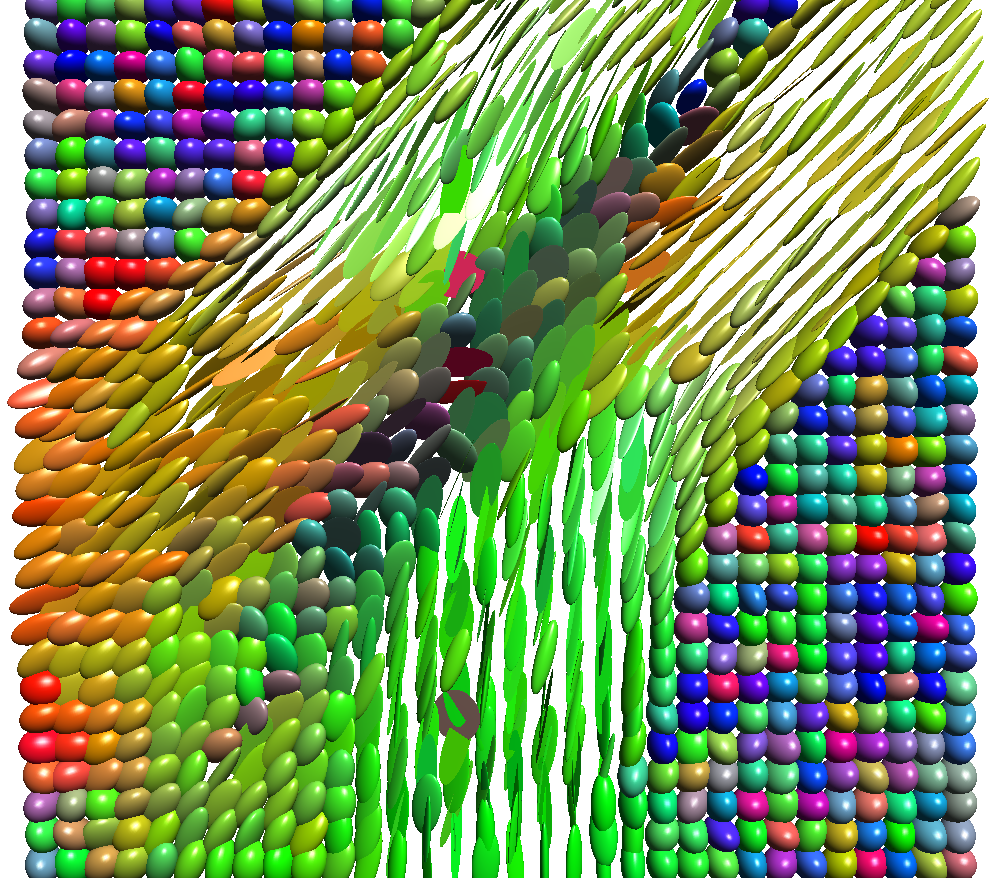
\includegraphics[width=0.5\linewidth]{./figures/experiments/noisy_dti32x32.png}
    }
    \subfloat[][Denoised]{
	\label{fig:application_dti1_denoised}
	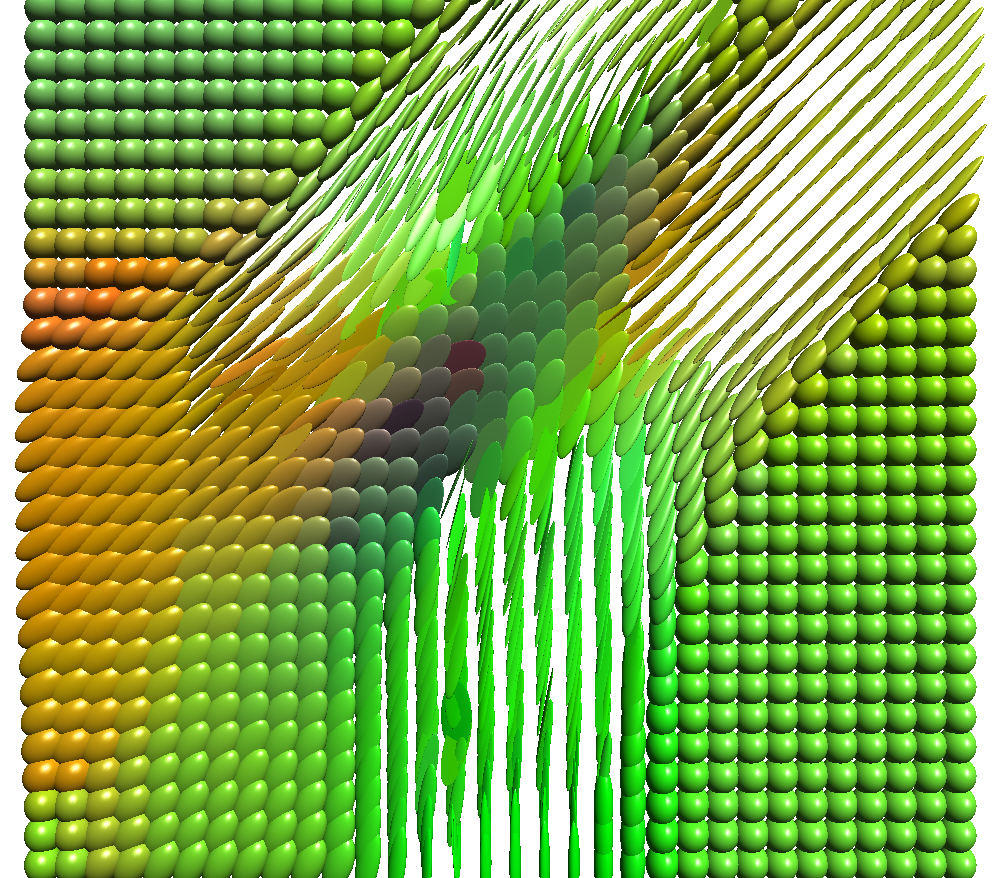
\includegraphics[width=0.5\linewidth]{./figures/experiments/denoised_dti32x32.png}
    }\\
    \caption[Denoising DT-MRI data]{Denoising a DT-MRI image with pixel in SPD(3)
	\subref{fig:application_dti1_noise} Original DTI data, 32x32 pixel
	\subref{fig:application_dti1_denoised} Denoised, IRLS with $\lambda=?$, $?$ IRLS steps, $?$ newton steps per IRLS step
	\label{fig:application_dti1}
    }
\end{figure}

In Figure \ref{fig:application_dti1} the IRLS minimizer is applied to DTI data set provided by Barmpoutis \cite{barmpoutis}.
On clearly identify regions of high anistropy in the picture, where the molecules are forced to diffuse in one preferred direction.
The areas dominated mainly by green spheres correspond to approximately isotropic diffusion which means that there are no obstacles like axons in the brain in the 
immediate proximity of the water molecules.\\


\FloatBarrier
\subsection{3D DT MRI data} % (fold)
\label{sub:3DDTMRIdata}
% subsection 3D DT MRI data (end)

Finally, in Figure \ref{fig:application_dti2_noise} we show a 3D DTI image.

\begin{figure}[h!]
    \centering
    \subfloat[][Noisy]{
	\label{fig:application_dti2_noise}
	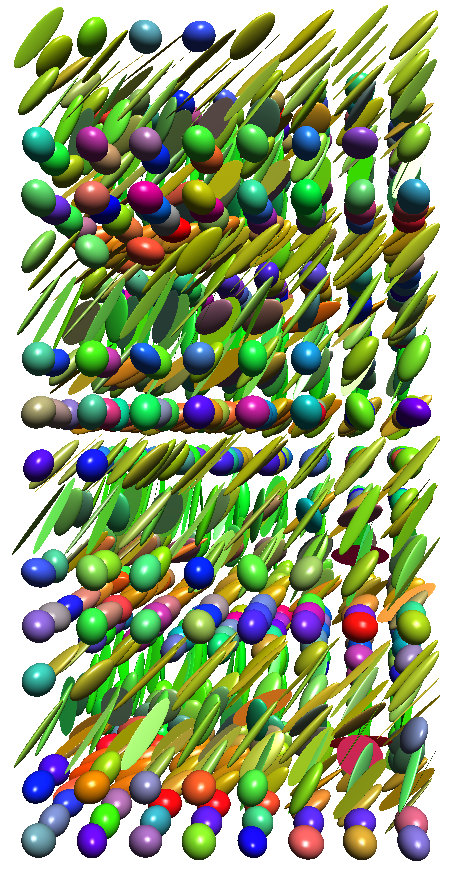
\includegraphics[width=0.4\linewidth]{./figures/experiments/noisy_dti3d8x16x16.png}
    }
    \subfloat[][Denoised]{
	\label{fig:application_dti2_denoised}
	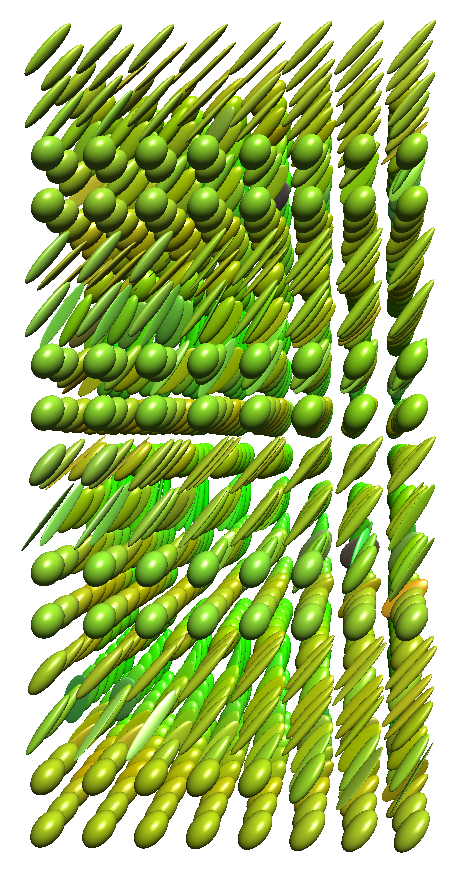
\includegraphics[width=0.4\linewidth]{./figures/experiments/denoised_dti3d8x16x16.png}
    }\\
    \caption[Denoising 3D DTI-MRI data]{Denoising a 3D DT-MRI image with pixel in SPD(3)
	\subref{fig:application_dti2_noise} Componentwise gaussian noise $\mu=0$, $\sigma=?$ added
	\subref{fig:application_dti2_denoised} Denoised, Proximal point with $\lambda=?$, 50 PRPT steps
	\label{fig:application_dti2}
    }
\end{figure}

% section SPD(3) image data (end)

\FloatBarrier
\section{Comparison IRLS and Proximal Point minimizers} % (fold)
\label{sec:Comparison IRLS and Proximal Point minimizers}

% section Comparison IRLS and Proximal Point minimizers (end)


\FloatBarrier
\section{Sensitivity to variations of the original data} % (fold)
\label{sec:Sensitivity}
%In section \ref{sub:Volume images} it was already mentioned that the computational and memory requirements become very demanding for increasing pixel numbers.
%If $N=XYZ$ denotes the number of pixels in the picture than the the number of non-zero entries in the Hessian is still $\mathcal{O}(N)$\\
In this section we perform a numerical experiment to see how changes of the noisy original picture influence the global solution found by the IRLS algorithm.
For that purpose we consider only the Brightness part of the Lena picture. In this grayscale image we pick a single non-zero pixel far enough in the inside of
the picture and set this pixel to zero, i.e. black color. This leads to two different original pictures
\begin{align}
    u_0,\hat{u}_0:\Omega &\to\mathbb{R}\\
    (\hat{u}_0)_{ij}&=\begin{cases}
	0, & \text{ if } i=i_0:=100,j=j_0:=10\\
	(u_0)_{ij}, &\text{else}
    \end{cases}.
\end{align}

Then for the original $u_0$ and the modified image $\hat{u}_0$ an IRLS minimization with $\lambda=0.1$, 5 iterations and one Newton step per reweighting is
performed to compare the two the solutions $u$ and $\hat{u}$. We take the absolute differences $e_{ij}=|u_{ij}-\hat{u}_{ij}|$ between the solutions
which leads to the error cone shown in Figure \ref{fig:experiment_sensitivity}\label{fig:experiment_sensitivity_plot}. This already suggests that the
error caused by changing the orginal data decays exponentially with distance $r=\sqrt{(i-i_0)^{2}+(j-j_0)^{2}}$.\\

After fitting a cone to the data, which is shown in \ref{fig:experiment_sensitivity}\label{fig:experiment_sensitivity_fit}
one finds that the aperture half-angle corresponds to a slope of $c=1.XXX$ such that the error will decay as
\begin{equation}
    e_{ij}=e^{-cr}.
\end{equation}

\begin{figure}[h!]
    \centering
    \subfloat[][Error cone]{
	\label{fig:experiment_sensitivity_plot}
	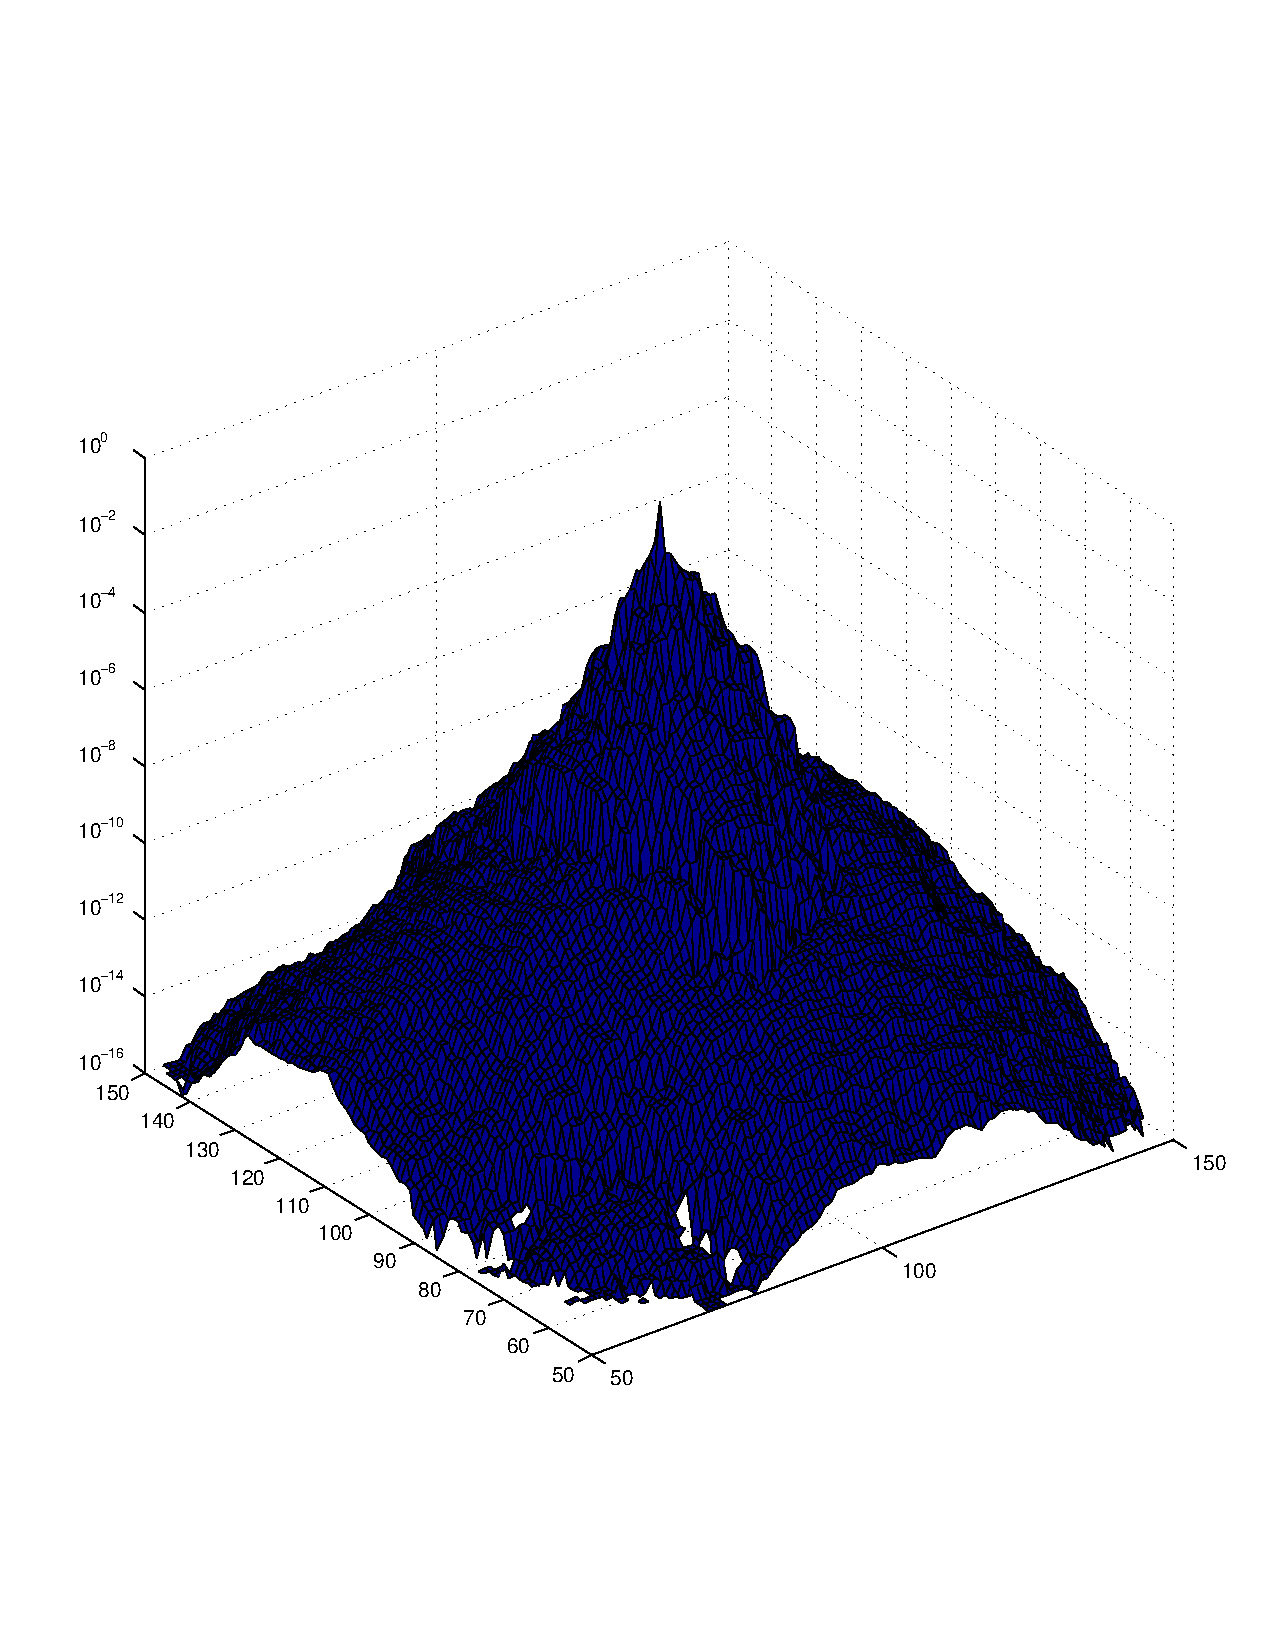
\includegraphics[width=0.4\linewidth]{./figures/experiments/cone.pdf}
    }
    \subfloat[][Fitted cone]{
	\label{fig:experiment_sensitivity_fit}
	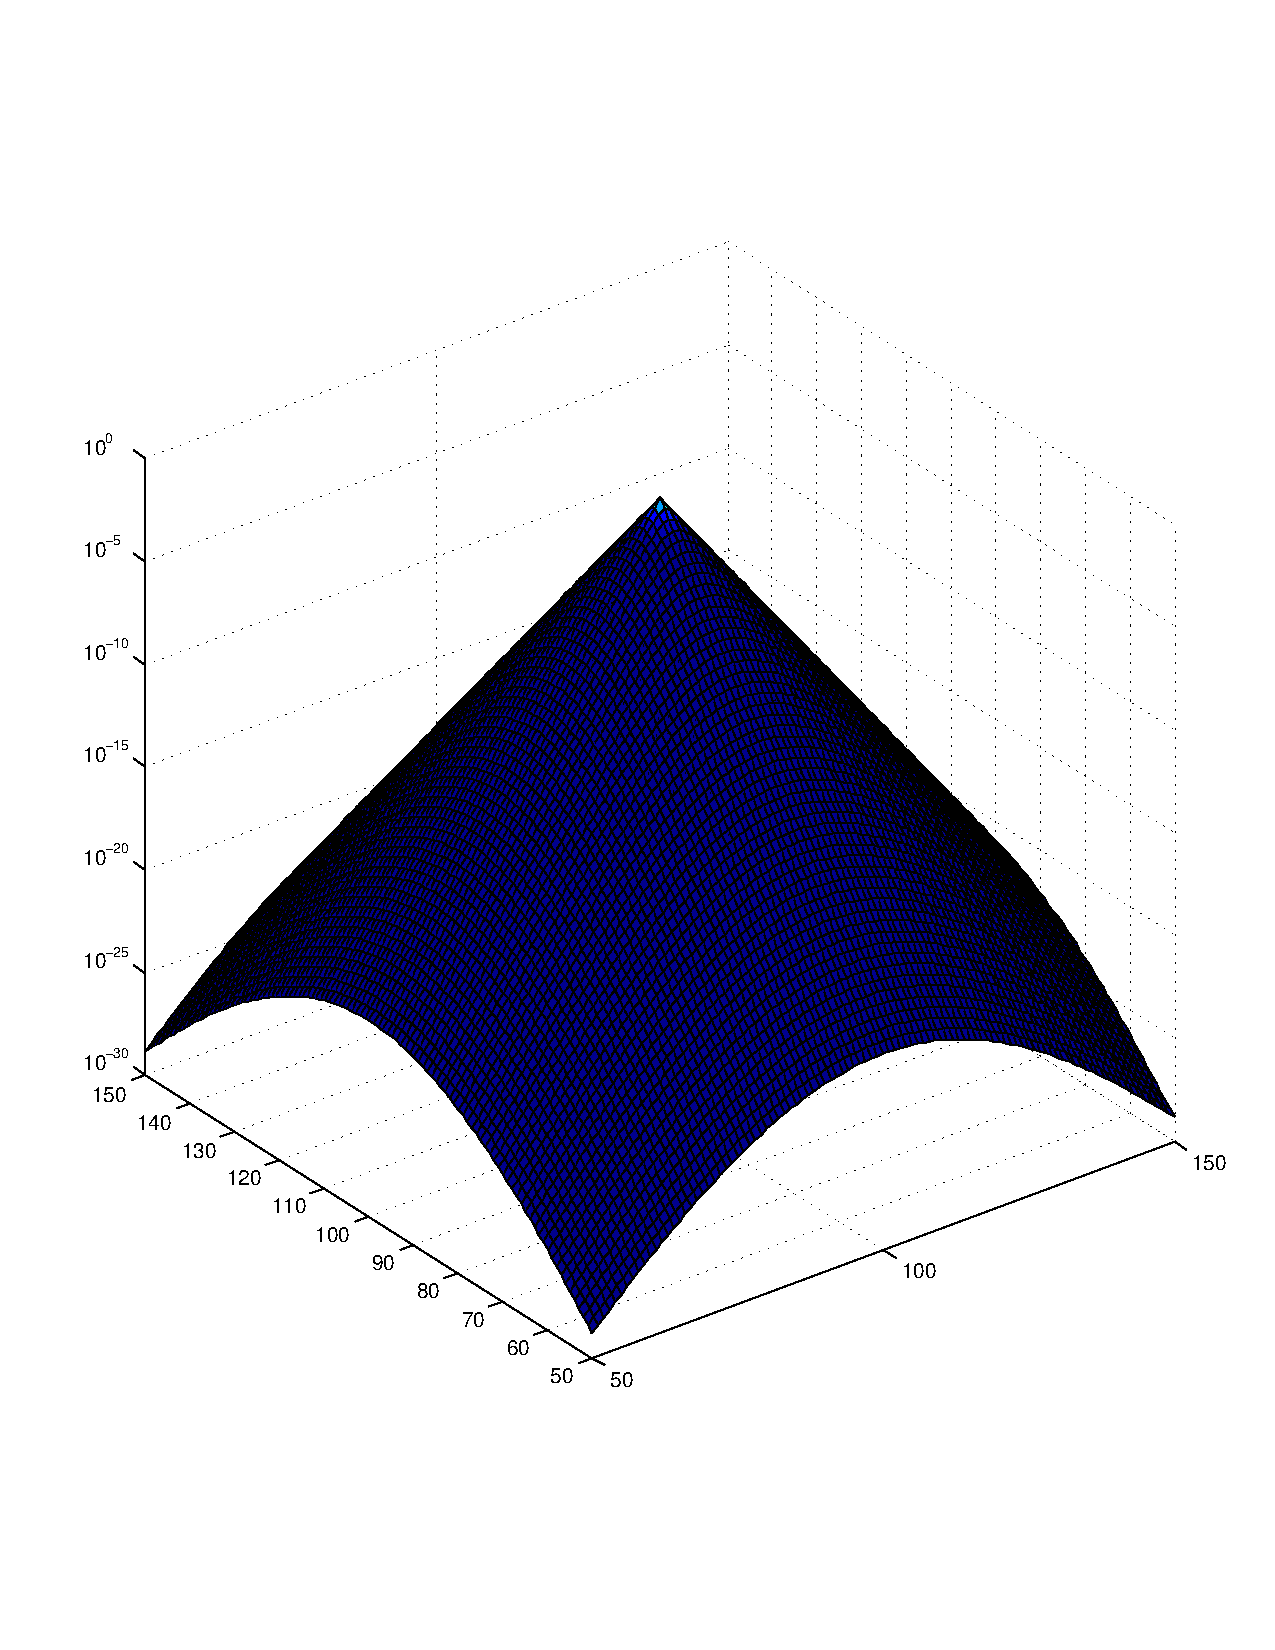
\includegraphics[width=0.4\linewidth]{./figures/experiments/fitted_cone.pdf}
    }\\
    \caption[Sensitivity to variation]{Sensitivity to change in original data
	\subref{fig:experiment_sensitivity_plot} Logarithmic plot of absolut differences $e_{ij}=|u_{ij}-\hat{u}_{ij}|$
	\subref{fig:experiment_sensitivity_fit} Cone fitted to the data, resulting in aperture half-angle of $\alpha=XXX$
	\label{fig:experiment_sensitivity}
    }
\end{figure}

The most important conclusion one can draw from this is that a pixel in the global minimizer depends practically only on a local neighborhood of that pixel
in the original picture, not on pixels far away from that neighborhood. We will discuss possible applications of this in section \label{sec:Recursivecomputationonsubdomains}.\\

Of course these findings should be verified analytically by providing sufficiently precise error bounds, which is, however, unfortunately out of the scope of this work.

% section Sensitivity to variations of the starting value (end)

\end{chapter}
